%!TEX root = ../main.tex
\chapter{Future $e^+e^-$ linear collider experiments}
\label{chap:FutureColliders}

Currently, the only high energy collider in operation is the \textit{Large Hadron Collider} (LHC) at CERN between Switzerland and France. The construction of the LHC started in 1995, was achieved in 2008 and its operation started in 2009. The LHC machine lies in a long underground tunnel of 27 km of circumference and is colliding protons at a center-of-mass energy up to $\sqrt{s} = 14$ TeV using supra-conducting magnets. It is probing the Standard Model to an unprecedented energy scale and search for unknown particles beyond the Standard Model. The discovery of the Higgs Boson in 2012 was one of the major milestone of the LHC. The colliding particles are protons which are composites particles, thus only a fraction of the energy is available during the collision. These collisions are very complex and make some measurements almost impossible at the LHC.

In the past, $e^+e^-$ colliders have been complementary tools to hadron colliders like the \textit{Large Electron-Positron Collider} (LEP) at CERN and Tevatron at Fermilab. A limitation of $e^+e^-$ ring colliders is the maximum achievable collision energy which is limited by the energy losses of the particles due to the synchrotron radiation. The synchrotron radiation power scales as
\begin{equation}
P_{synchrotron} \propto \frac{E^4}{R \times m^4}
\end{equation}
with $E$ the particle energy, $m$ the mass of the particle and $R$ the accelerator radius. The mass dependence makes the radiation losses significantly higher than protons. The maximum energy achieved by a $e^+e^-$ ring collider was of around a center-of-mass energy of $\sqrt{s} = 210$ GeV with the LEP. In this conditions, around 8 MW of energy is lost by synchrotron radiation.
Therefore, it is most likely that the next $e^+e^-$ collider will be a linear accelerator to achieve energies near the TeV scale.

The \textit{International Linear Collider} (ILC) and The \textit{Compact Linear Collider} (CLIC) are two proposed particle physics accelerator complementary to the LHC. The ILC is designed to collide electrons and positrons at a center-of-mass energy between 250 GeV to 500 GeV with a possible upgrade to 1 TeV. The advantage of the ILC is that it provides a reduced background and cleaner events compared to a hadron collider thus allowing for high precision measurements. The following section will give a short summary of the ILC machine and its detectors and based on the ILC Technical Design Report (TDR) \cite{ILC_TDR_Vol1, ILC_TDR_Vol2, ILC_TDR_Vol3.1, ILC_TDR_Vol3.2, ILC_TDR_Vol4}.

\section{The International Linear Collider}
\label{sec:ILC}

The International Linear Collider (ILC) is a planned 31 km long $e^+e^-$ linear collider to be build in Japan with a design peak luminosity of around $2 \times 10^{34} cm^{-2}s^{-1}$ and a center-of-mass energy of 500 GeV. An upgrade up to 1 TeV center-of-mass energy and a higher luminosity is possible. Polarization up to 80\% for electrons and 30\% for positrons can be achieved enabling the enhancement of rates and the reduction of SM background. The polarization is a crucial ingredient in the ILC program. It uses supra-conductive RF (SCRF) cavities to accelerate electrons and positrons. The project is currently under discussion between the governments and a decision by the end of 2018 should be reached. A schematic of the ILC layout is shown in figure \ref{fig:ILC_schematic}.

\begin{figure}[htbp!]
  \centering
  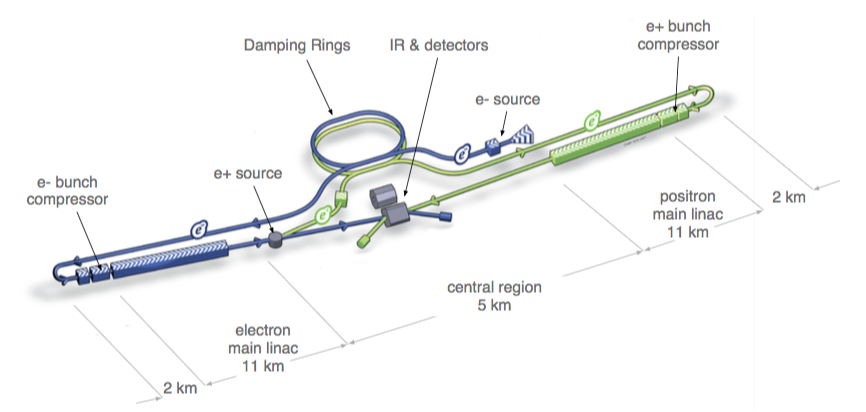
\includegraphics[width=0.7\linewidth]{chap2/fig/ILC_schematic.png}
  \caption{Schematic of the International Linear Collider (not to scale). Taken from \cite{ILC_TDR_Vol1}.} \label{fig:ILC_schematic}
\end{figure}

The electron beam is produced by a laser illuminating a photocathode of GaAs in a DC gun. It provides the bunches of electrons with a polarization of 90\%. The bunches are accelerated to 5 GeV in a SCRF booster before being collected in the dumping ring. The dumping ring has a circumference of 3.2 km where bunch trains are formed and the emittance of the beam reduced by 5 orders of magnitude to 20 nm. It is achieved by the succession of normal magnets, supra-conducting magnets and wiggler magnets. The wiggler magnets cool the beam by dumping synchrotron radiation thus reducing the beam emittance. The bunch trains formed by the ring are around 200 ms apart containing more than 1000 electron bunches.

The electron beam is then transported by the Ring to Main Linac (RTML), accelerating electrons from 5 GeV to 15 GeV while compressing the bunch-length to few micrometers required by the integration region (IR).

The main linacs of the ILC accelerate the electron beam up to 250 GeV by using supra-conductive RF cavities of niobium operated at 2 Kelvins housed in cryomodules. The RF power is delivered by a system of Klystrons. The average gradient of the cavities is around 31.5 $\frac{MV}{m}$ with a quality factor $Q_0 \geqslant 10^{10}$. The synchrotron sources of FLASH and recently of the European X-Ray Free Electron Laser (XFEL) based at DESY, are a demonstration of the mass-production and operation of cryomodules which represents around 1\% of the ILC.

After the acceleration, the electron beam is transported through a supra-conducting helical undulator which generates photons between 10 to 30 MeV. Then the electron beam is separated from the photon beam and transported by the Beam Delivery System (BDS) to the IR. The BDS focuses the beam down to 474 nm $\times$ 5.9 nm (x and y respectively at $\sqrt{s} = 500$ GeV) to reach the luminosity goal of $2 \times 10^{34} cm^{-2}s^{-1}$.

The photons are directed onto a thin ($0.4 X_0$) titanium alloy (Ti) target producing electrons-positrons pairs. The positrons are accelerated to 400 MeV in a first step while the remaining electrons and photons are dumped. The positrons are accelerated to 5 GeV by a booster and injected into a dumping ring, parallel to the electron ring. From there, the positron beam follows a similar beam line as the electron beam and both beams are brought into collision at the IR, where two detectors lie that can be operated in push-pull configuration.

\begin{figure}[htbp!]
  \centering
  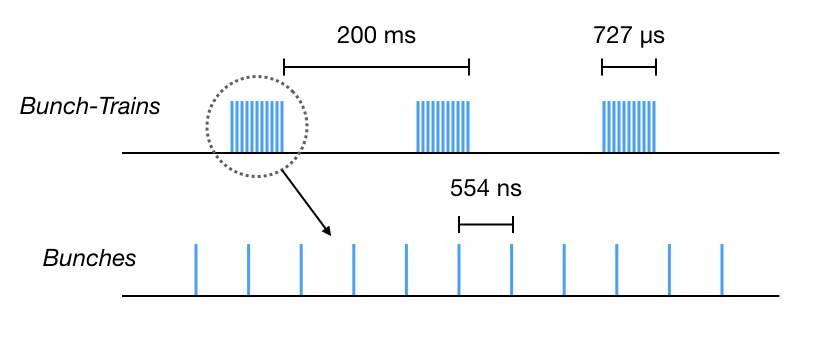
\includegraphics[width=0.7\linewidth]{chap2/fig/BeamStructure.jpeg}
  \caption{Schematic of beam structure of the ILC operated a design parameters.} \label{fig:ILC_BeamStruct}
\end{figure}

The beam structure of the ILC consists of bunch-trains of 1312 bunches of $2 \times 10^{10}$ particles each and separated by around 550 ns. The distance between bunch-trains is around 200 ms corresponding to a 5 Hz repetition frequency (up to 10 Hz depending on the running scenario). A schematic of the beam structure is shown in figure \ref{fig:ILC_BeamStruct}.

The CLIC concept \cite{CLIC_CDR} is drastically different in the design and technology used. CLIC uses normal conducting copper cavities operated at 12 GHz much higher than ILC (1.3 Ghz). It uses a two beam operation scheme where a high current, low energy drive beam provides RF power to accelerate a low current, high energy beam. By this mean, a center-of-mass energy up to $\sqrt{s} = 3$ TeV could be achieved. The CLIC technology is yet not mature compared to the ILC and still needs several years of R\&D before a full CLIC accelerator could be constructed.

\section{The International Large Detector (ILD)}
\label{sec:ILD}

The physics program of the ILC is quite ambitious. In order to realize it, significant advances in detector performance is essential. The detector concepts for the ILC are focused on the \textit{Particle Flow} approach. The Particle Flow approach is discussed in section \ref{sec:PFA}. It is aiming to reconstruct individually each particles in an event. This requires an unprecedented spacial resolution in all sub-detectors to efficiently separate charged and neutral particles even within jets. This motivates for a highly efficient tracking system and highly granular calorimeters but also a sophisticated reconstruction software.

At the ILC, it is planned to have two detector experiments sharing the interaction region in a push-pull configuration. One detector occupies the IR while the other detector is parked in the detector hall. Both detectors can be moved in and out of the IR periodically every few weeks. Two detector concepts have been developed in the ILC Technical Design Report \cite{ILC_TDR_Vol4}, the \textit{Silicon Detector} (SiD) and the \textit{International Large Detector} (ILD). A detailed detector simulation is available for both of the concepts and has been used extensively in the study of the potential of ILC physics as well as detector optimizations. The detectors concepts contain realistic implementations of all sub-detectors and have been cross-checked with prototype data if possible (see chapter \ref{chap:CALICE_Det}). In the following, the ILD detector will be briefly described.

The ILD detector is a multi-purpose detector. The tracking system and the calorimeter systems are both located within a supra-conducting solenoid magnet of 3.4 m radius providing a field of 3.5 T parallel to the beam axis. Schematics of the ILD detector can be seen in figure \ref{fig:ILD}.

\begin{figure}[htbp!]
  \centering
  \begin{subfigure}[t]{0.49\textwidth}
    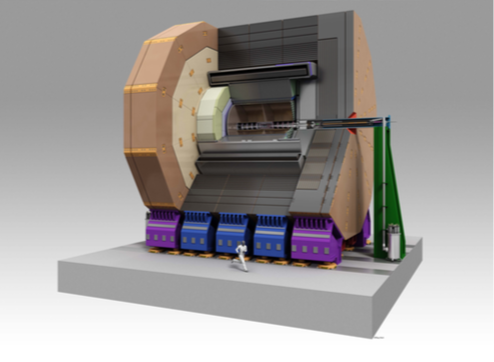
\includegraphics[width=1.\linewidth]{chap2/fig/ILD_full.png}
  \end{subfigure}
  \hfill
  \begin{subfigure}[t]{0.49\textwidth}
    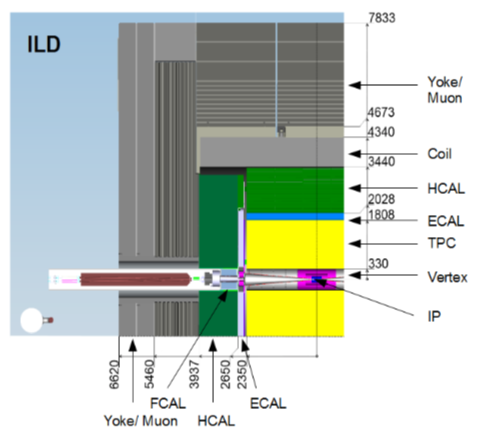
\includegraphics[width=1.\linewidth]{chap2/fig/ILD_layout.png}
  \end{subfigure}
  \caption{Schematic views of the ILD detector. Dimensions on the right figure are in mm. \cite{ILC_TDR_Vol4}.} \label{fig:ILD}
\end{figure}

\subsection{ILD Tracking System}

\subsection{ILD Calorimeter System}

\section{ILC Physics}
\label{sec:ILC_Physics}

\subsection{Higgs Physics}
\subsection{Electroweak Physics}
\subsection{Top mass measurement}
\subsection{Beyond the Standard Model}
